\chapter{Prototype Design}
\label{chap:prototype}

\section{Overview}

In this chapter the progression of the Rapidly Reconfigurable Research Cockpit prototype is described.
Three major versions of the prototype are outlined here and explained how they evolved from each other.
The first prototype was not used in a formal experiment, but two versions based on the second prototype were used for Experiment 1 (Chapter \ref{chap:pointing}) and 2 (Chapter \ref{chap:ph_exp}).
The final prototype was used in the third experiment (Chapter \ref{chap:de_exp}).

\section{Requirements}

In this section, the requirements we developed for the Rapidly Reconfigurable Research Cockpit (R3C) prototype are outlined.
These requirements guided the development of the prototypes, based on the technology available.

\begin{description}
    \item [Rapid prototyping of physical mockup.]
        The main motivation for this system is that it enables rapid redesign of cockpit systems undergoing design evaluations.
        To permit this, the R3C system should allow for rapid changes in the physical world without needed to reconfigure the software heavily, or reconfigure any hardware for interaction.
    \item [Minimal setup and calibration.]
        Another goal of the system is that it can be used ``on top'' of existing mockup systems.
        One consequence of this means that as much as possible, the hardware used must be easy to set up and able to use in constrained spaces.
        This eliminates some of the high-end head mounted displays that use complicated head tracker systems requiring precise calibration.
        Additionally, this eliminates many of the past approaches to hand tracking which use multiple cameras precisely calibrated, or magnetic sensors in a well-defined magnetic field.
        The minimal setup also leads to the need for hand tracking, as the recognition of the user input must be done without outfitting the mockup with working input actuators (i.e.\ buttons).
    \item [Immersive head mounted display.]
        The visual system needed.
    \item [Unobtrusive hand tracking.]
        The hand tracking.
\end{description}

\section{Prototype Development}

\subsection{First Prototype}

The first prototype was the proof of concept of the system, and before it could be used for research studies, it was quickly outdated with new technology and updates.
It utilized the first generation Oculus Rift Development Kit and the first generation of software for the LeapMotion hand tracker.

\subsubsection{VR Headset and Visuals}

\subsubsection{Hand Tracking}

The LeapMotion hand tracker was selected as 

\subsubsection{Button Recognition}

With a working hand tracking system, the next step was to develop a method to determine when users were pushing a button.
The button recognition system was developed within the EDGE engine agnostic to the hand tracker, so that future prototypes could use a different hand tracker if a new device were released.
The 

\subsubsection{Challenges}

The hand tracking caused two issues with the use of the prototype.
The first was simply that the reliability of the tracking caused many dropped .

\begin{itemize}
    \item First generation Oculus prototype
    \item No head tracking on visuals
    \item Hand tracking was primitive but worked
    \item No full hand skeleton tracking, just fingertips
    \item Button recognition alogrithm developed
    \item challenges were hand tracking registration and visuals
    \item Sound with button recognition
\end{itemize}

\subsection{Second Prototype}

A number of improvements were made in the second generation of the prototype.
Due to software upgrades, the hand tracking became more robust and provided more complete information about the entire hand position.
The visuals were upgraded to the second Development Kit of the Oculus Rift, which provided improved visual resolution but more importantly an external head tracker (camera) which enabled head movement and virtually eliminated drift of the internal sensors.
A major focus of this version of the development work for this prototype was to improve reliability and registration.
The reliability was partially improved with the new hand tracking software, but other countermeasures developed are described as well.
Registration refers to the alignment between the physical world and the virtual world.
%An important aspect of our system is that the physical world is providing an overlay 

\subsubsection{Hand Tracking}

The upgrade to the hand tracking software provided two features that were integrated.
The first was an improvement in the fidelity of the tracking, including full information on the joints of the hand.
The second was the introduction of a ``head mounted'' mode, which allowed for tracking to be optimized for looking down at a hand.

The tracking upgrade allowed us to access the location and orientation of the entire hand and each segment of each finger.

The head-mounted mode was introduced to provide hand position in a virtual environment by way of mounting it on the head-mounted display itself.
Upon initial testing of this feature, two observations were made.
The tracking was much improved when looking down at the hands, seemingly providing more robust and reliable tracking data.
However, using it mounted to the head-mounted display caused a larger disconnect between the real world and physical world.
The registration relies on a known, rigid connection between the hand tracker and the location of the instruments.
When the tracker was mounted on the head-mounted display, the transformation between LeapMotion coordinates and panel coordinates relied on knowing the location of the head.
Although this information could be obtained from the newer model HMD which included head tracking, it was simply not precise or stable enough to use as the base for the hand tracking coordinates.

This led us to develop a mount that would hold the LeapMotion upside down over the panel and instruments.

\subsubsection{Capacitive Touch Sensors}

The capacitive touch sensors were initially developed as a countermeasure to the problems encountered with the hand tracking from the original prototype.
As the hand tracking became more robust with the new software from the manufacturer, the countermeasure was not as important, but the sensors played a new role in the prototyping: validating the accuracy and providing calibration for the hand tracker.

In order to be able to activate the buttons reliably when the hand tracking was degraded or dropping out, it was decided to investigate capacitive touch sensors.
To stay with the goal of minimal setup, the original capacitive touch sensors were developed with copper tape electrodes placed on the top of the 3D printed instrument buttons.
These electrodes are shown in Figure \ref{fig:proto_notsure}.
An MPR121 capactive touch sensor was used to read the electrodes and communicate with an Arduino which sent touch events over a serial communication line to the computer.
These serial events were read by the rendering engine to trigger events when a copper pad was touched.


\subsubsection{Calibration}

The hand tracking provided by the LeapMotion provided precise and repeatable measurement of the hand positions throughout its tracking volume.
The accuracy as the hand got further away from the sensor, however, was insufficient.
Put another way, the position of the hand in the virtual world was offset from the true button position in the physical world, yet the offset was consistent between movements.
This led us to develop a calibration to provide a more accurate registration between the virtual and physical hand positions.
First, the mathematical basis for this calibration is described, then the integration with the prototype is explained.

Since we accurately know the position of the panel and instruments, it is only required to solve the following linear algebra equation for the transformation matrix, $\mathbf{T}$:
\begin{equation}
    \vec{x}_{known} = \mathbf{T}\vec{x_{measured}}
    \label{eq:proto_Tvec}
\end{equation}

Using a simple least squares approach to find the coefficients of the matrix, the registration between the virtual and physical worlds is vastly improved.
The transformation matrix is not constrained to a simple rotation (i.e.\ not assumed orthogonality or other special properties) so the solution is found by expanding and solving the general homogenous coordinates transformation matrix.

\begin{equation}
    \begin{bmatrix}
        x_{known} \\
        y_{known} \\
        z_{known} \\
        1
    \end{bmatrix} =
    \begin{bmatrix}
        T_{11} & T_{12} & T_{13} &T_{14} \\
        T_{21} & T_{22} & T_{23} &T_{24} \\
        T_{31} & T_{32} & T_{33} &T_{34} \\
        0 & 0 & 0 & 1
    \end{bmatrix}
    \begin{bmatrix}
        x_{measured} \\
        y_{measured} \\
        z_{measured} \\
        1
    \end{bmatrix}
    \label{eq:proto_Tmat}
\end{equation}

Typical least squares approaches would attempt to find $\mathbf{x}_{measured}$ in Eqn.\ \ref{eq:proto_Tvec}, however we desire to find the matrix T itself.
It can be shown that expanding the matrix equation (Eqn.\ \ref{eq:proto_Tmat}) for multiple points (i.e.\ $\vec{x}_{known,1},\dots,\vec{x}_{known,n}$ and $\vec{x}_{measured,1},\dots,\vec{x}_{measured,n}$) and then collecting like terms will convert the problem into three different least squares problems.
They are shown here, dropping the subscripts to $k$ and $m$ for known and measured.

\begin{gather*}
    \begin{bmatrix}
        x_{k1} \\
        x_{k2} \\
        \cdots \\
        x_{kn}
    \end{bmatrix}
    =
    \mathbf{X}_M
    \begin{bmatrix}
        T_{11} \\
        T_{12} \\
        T_{13} \\
        T_{14}
    \end{bmatrix}
    ,\;\;
    \begin{bmatrix}
        y_{k1} \\
        y_{k2} \\
        \cdots \\
        y_{kn}
    \end{bmatrix}
    =
    \mathbf{X}_M
    \begin{bmatrix}
        T_{21} \\
        T_{22} \\
        T_{23} \\
        T_{24}
    \end{bmatrix}
    ,\;\;
    \begin{bmatrix}
        y_{k1} \\
        y_{k2} \\
        \cdots \\
        y_{kn}
    \end{bmatrix}
    =
    \mathbf{X}_M
    \begin{bmatrix}
        T_{31} \\
        T_{32} \\
        T_{33} \\
        T_{34}
    \end{bmatrix}
    ,\\
    \text{where}~\mathbf{X}_M =
    \begin{bmatrix}
        x_{m1} & y_{m1} & z_{m1} & 1 \\
        x_{m2} & y_{m2} & z_{m2} & 1 \\
        &\dots & & \\
        x_{mn} & y_{mn} & z_{mn} & 1
    \end{bmatrix}
\end{gather*}

At least 4 points are needed to solve this system, and it has been found that a calibration with small least squares residuals can be achieved with 10-20 well chosen points.
The calibration matrix is then used to find the offset of the tip of the index finger for each hand, and this offset is used to move the entire hand.


\subsubsection{Capacitive Touch Arrays}

This would help to determine if we had any registration biases in our system.
To accomplish this, a custom printed circuit board was developed that provides an electrode array of 5 rows and 5 columns over a 1-inch by 1-inch square.
This board is show in Figure \ref{fig:pe_capacitive}, where it is mounted in a 3D printed instrument.
The capacitive state of each row and column can provide a measurement of the center of the finger press on the grid created by the rows and columns.
With this configuration finger-location accuracy of under 0.1-inch can be achieved.
The location of the finger press can help provide a measure of the accuracy of the registration between the optical sensors and the real world location.

\begin{figure}
    \centering
    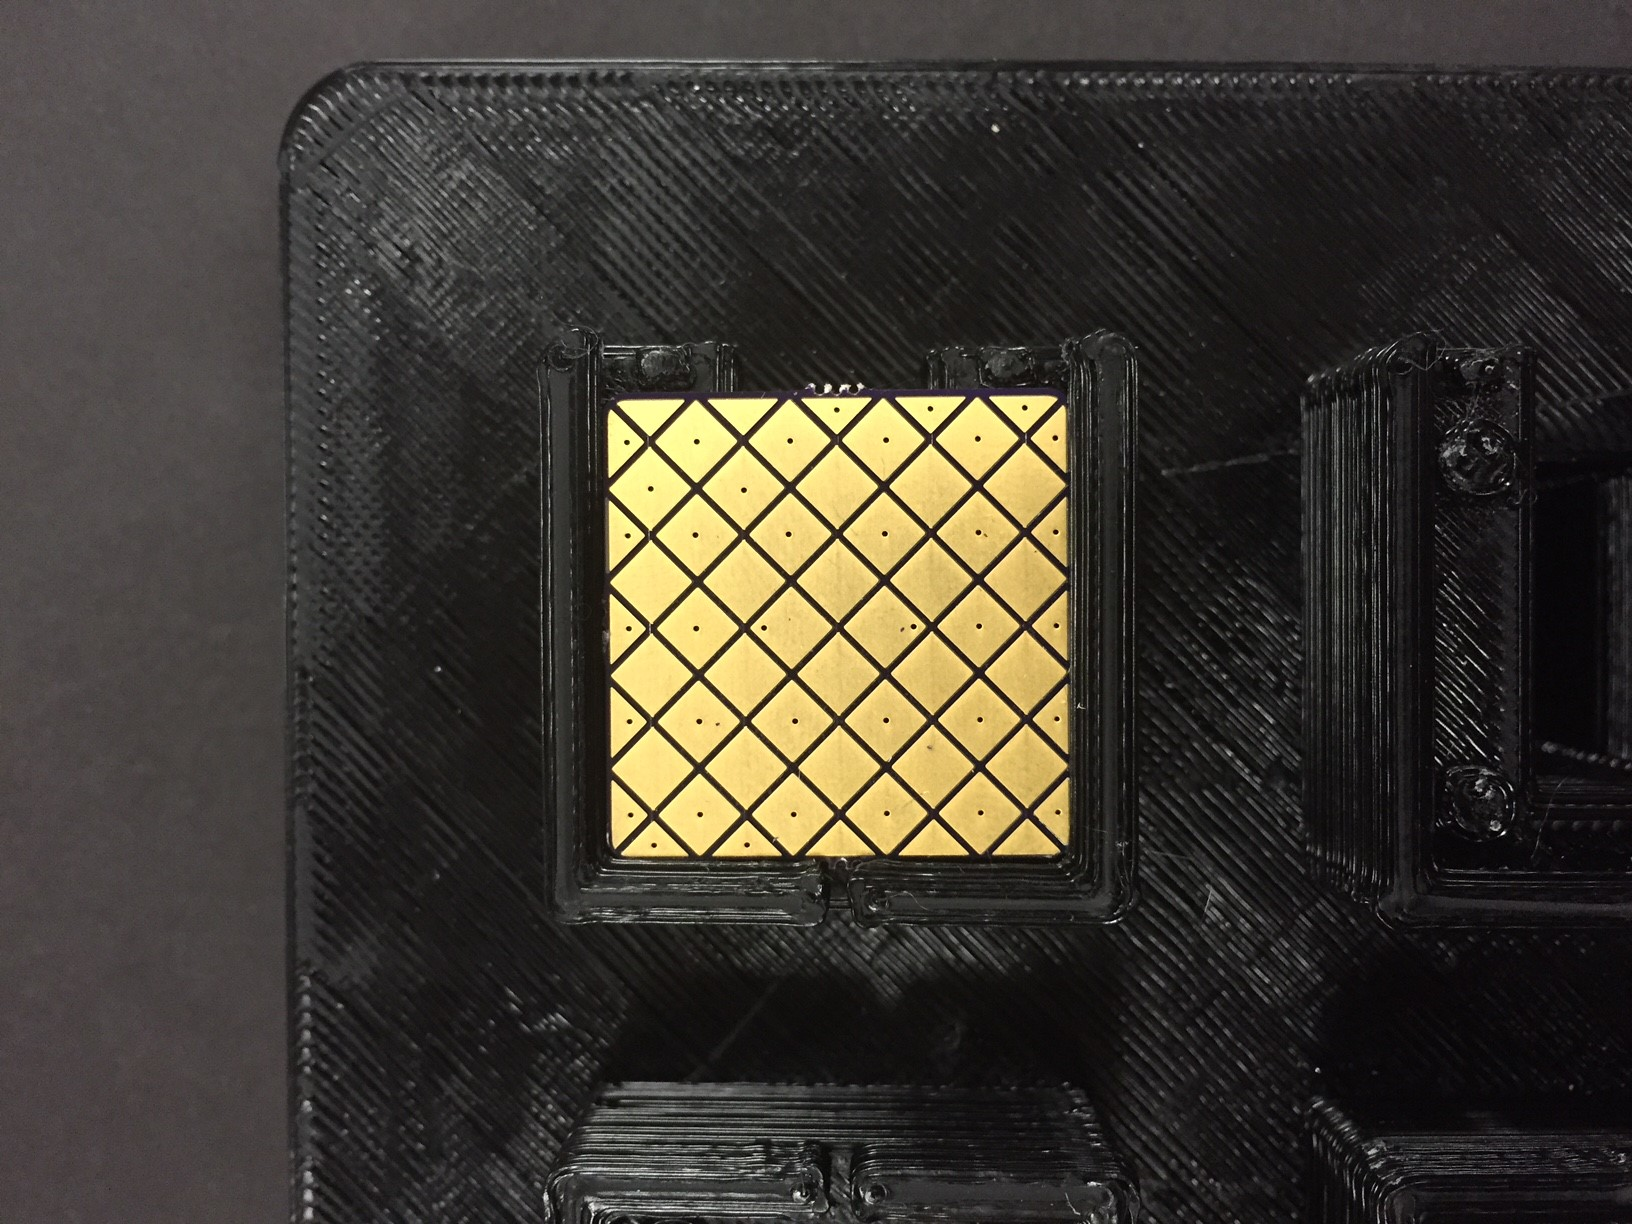
\includegraphics[width=1.25in]{pe_capacitive.jpg}
    \caption{Capacitive touch array button. Each row and column of diamond pads are connected as one electrode each and together can provide location information of where the user presses.}
    \label{fig:pe_capacitive}
\end{figure}

\begin{itemize}
    \item second generation Oculus prototype
    \item Big upgrade due to head tracking
    \item Hand tracking software upgrade allowed us to track the whole hand
    \item .Capacitive touch developed --first as big pads on each button
    \item .Capactiive touch sensor pads which allowed measurement of accuracy
    \item .Led to development of calibration mechanism
    \item Hand tracking upside down vs right side up led to moving the tracker
\end{itemize}

\subsection{Final Prototype}

\begin{itemize}
    \item Return to pure 3d printed instruments
    \item Calibration with touchscreen
    \item Calibration on a single plane problem
\end{itemize}

\section{Lessons Learned and Future Work}

\begin{itemize}
    \item IR interference
    \item Small amounts of training make a big difference
    \item Conversely, not explaining fully how it works can lead to good performance/feedback
    \item hand tracking difficulties can be very frustrating
\end{itemize}
